\documentclass{beamer}
\usetheme{metropolis}
\usepackage[utf8]{inputenc}
\usepackage[estonian]{babel}
%\usepackage[english=british]{csquotes}
\usepackage[autostyle=false]{csquotes}
\usepackage{multirow}

\usepackage[normalem]{ulem}

\title{IDU1321. Ettevõtte äriarhitektuur}
\subtitle{Kaheksas loeng}
%\date{10.09.2017}
\author{Andres Kütt}
\institute{Arhitekt}


\begin{document}

\begin{frame}
\titlepage
\end{frame}

%\begin{frame}[standout]
%Eksami kuupäev?
%\end{frame}

\begin{frame}[standout]
Küsimusi kodutöö kohta?
\end{frame}


\begin{frame}{Kus me oleme?}
	\begin{center}
		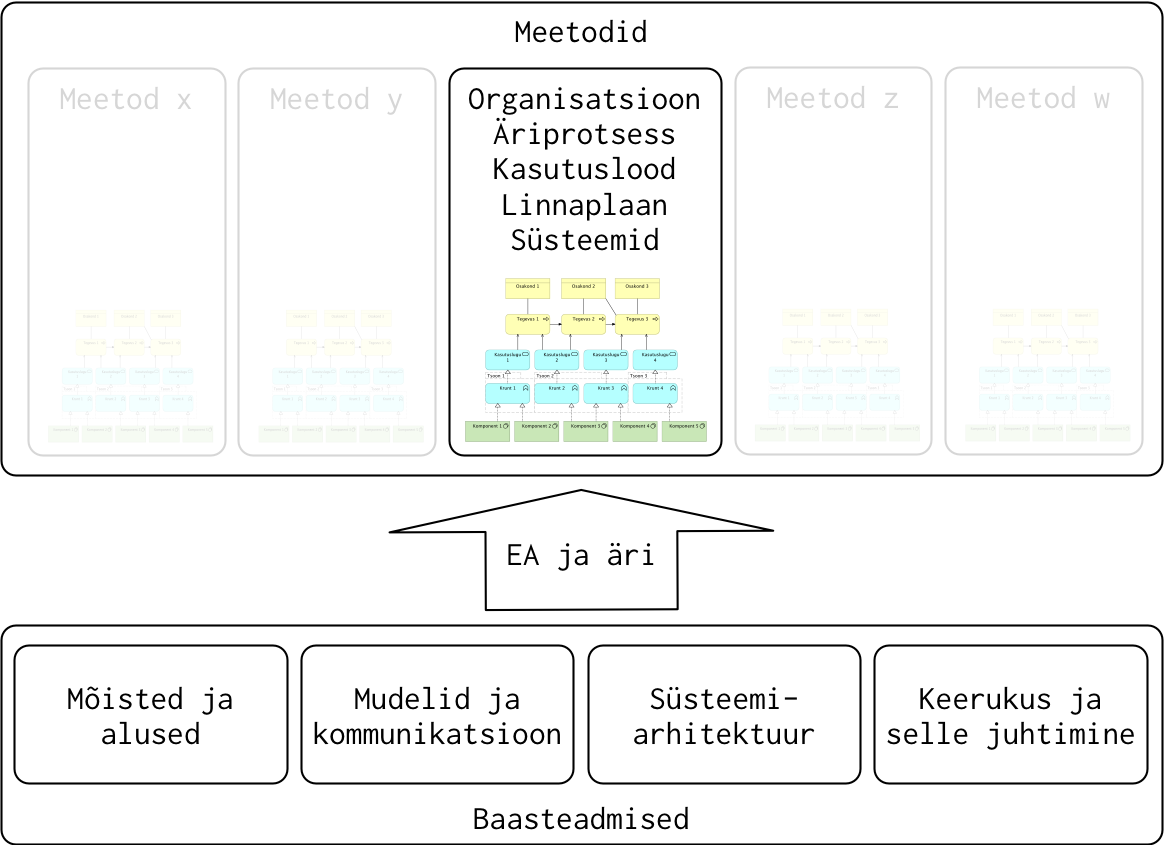
\includegraphics[width=.8\textwidth]{aine_struktuur}
	\end{center}
\end{frame}

\begin{frame}[fragile]
  \frametitle{Keerukuse mõiste}
  Ühest definitsiooni ei ole. On viisid selle mõõtmiseks \cite{mitchell2009complexity}:
	\begin{itemize}
		\item Keerukus kui suurus, osiste ja nendevahelise seoste hulk
		\item Keerukus kui entroopia määr
		\item Keerukus kui pakitavuse määr
		\item Keerukus kui loogiline või termodünaamiline sügavus
		\item Keerukus kui sisendi ja väljundi seos
		\item Keerukus kui fraktaaldimensioon
		\item Keerukus kui alamsüsteemide hulk
		
	\end{itemize}
\end{frame}

\begin{frame}{Staatiline ja dünaamiline keerukus}
	\begin{center}
		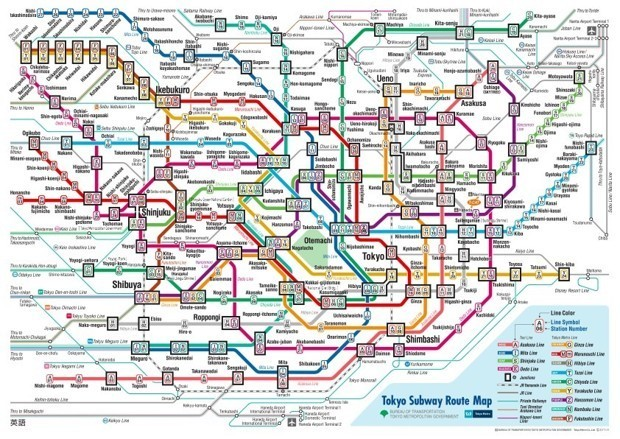
\includegraphics[width=\textwidth]{tokyo_subway}
	\end{center}
\end{frame}

\begin{frame}{Staatiline ja dünaamiline keerukus}
	\begin{center}
		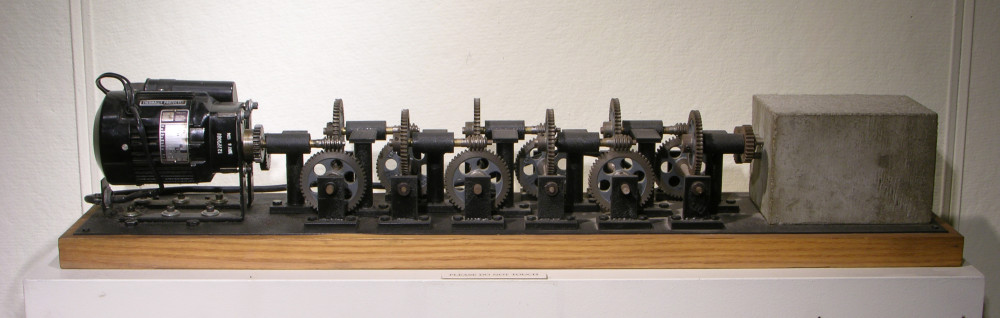
\includegraphics[width=\textwidth]{arthur-ganson-machine-with-concrete-1992}
	\end{center}
Arthur Ganson. Machine With Concrete
\end{frame}

\begin{frame}{Keerulisus (complicatedness)}
	\begin{center}
		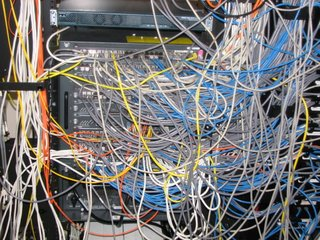
\includegraphics[width=.6\textwidth]{complicatedness}


Keerulisus on asjade omadus näida keeruline

	\end{center}
\end{frame}

\section{Kolm keerukuse omadust}
\begin{frame}[fragile]
	\begin{center}
		\LARGE{\textbf{Järgnevas kasutame üht konkreetset definitsiooni}}
		\\[4cm]
		\small{MITis leiutatud. Mõnevõrra matemaatiliselt keeruline kuid reaalses elus valideeritud. https://goo.gl/gPtX6F}
	\end{center}
\end{frame}

\begin{frame}{Keerukus ajab hinda üles}
\center{	$keerukus_a=keerukus_b\times k \Rightarrow hind_a=hind_b\times k^{1.4}$}
	\begin{itemize}
		\item Keerukus ajab R\&D kulusid üles astendajaga 1.4
		\item 20\% keeruksue vähenemist tähendab hinna vähenemist 29\% võrra sest $1.2^{1.4}\approx1.29$
		\item \textbf{Järeldus:} keerukuse vähendamisse tasub investeerida
	\end{itemize}
\end{frame}

{
\usebackgroundtemplate{\includegraphics[width=\paperwidth]{complexity_feedback}}
\begin{frame}[plain]
\end{frame}
}

\begin{frame}{Keerukuse kasv ja meie võimed}
	\begin{center}
		\includegraphics[width=\textwidth]{keerukus}
	\end{center}
\end{frame}


\section{Harjutus}
\begin{frame}{Hindame asjade keerukust}

	\begin{itemize}
		\item Järjestage järgmised süsteemid staatilise (tükid, nende liigid, liidesed ja nende liigid) ning dünaamilise keerukuse (võime keeruliselt käituda) järgi
		\begin{enumerate}
			\item Jalgrattakett
			\item Kolm raudkuuli avakosmoses
			\item Vann vett
			\item Rolex Submariner
			\item Vox AC15
			\item Intel Coffee Lake põlvkonna mikroprotsessor
		\end{enumerate}
		\item Tegutsege paarides
		\begin{itemize}
			\item 18 minutit tööd süsteemide kallal
			\item 12 minutit esitlete oma tulemust kõrvalpaarile ja kuulate nende oma: \textbf{Kirjutage üles erinevus positsioonides}
		\end{itemize}
	\end{itemize}
\end{frame}

\begin{frame}{Minu tulemus}
\begin{table}[]
\centering
\begin{tabular}{l|l|l|l}
 & \textbf{Staatiline} & \textbf{Dünaamiline} & \textbf{Vahe} \\ \hline
Vann  vett & 1 & 8 & -7 \\
Kolm keha & 2 & 9 & -7 \\
Jalgrattakett & 3 & 7 & -4 \\
Vox AC15 & 3 & 5 & -2 \\
Rolex Submariner & 8 & 1 & 7 \\
Arvutiprotsessor & 9 & 3 & 6
\end{tabular}
\end{table}
\end{frame}

\begin{frame}{Harjutuse kokkuvõte}
	\begin{itemize}
		\item Kas teie vahed tulid sama suured?
		\item Millest tulevad erinevused hinnangutes?
		\item Millist teadmist vajas keerukuse hindamine?
	\end{itemize}
\end{frame}

\begin{frame}{Kordame}
	\begin{itemize}
		\item Keerukus on laialivalguv teema, tema mõõtmine väga harva praktiliselt teostatav 
		\item Keerukuse alla viimisel on kuludele oluline mõju
		\item Keerukusel on komme ennast ise toita, sellest tuleneb eksponentsiaalne kasv
		\item On lihtne sattuda teisele poole oma võimete piiri
	\end{itemize}
\end{frame}

\begin{frame}{Järgmine kord}
\begin{center}
Sööme kõik kodus piparkooki
\end{center}
\end{frame}

\begin{frame}{Bibliography}
	\bibliographystyle{plainnat}
	\bibliography{idu1321}
\end{frame}

\begin{frame}[standout]
Aitäh!
\end{frame}

\end{document}
